\documentclass[dvipdfmx,11pt]{beamer}
\usepackage{lipsum}
\usetheme{Verona}
\usepackage{bxdpx-beamer}
\usepackage{pxjahyper}
\usepackage{minijs}
\usepackage{mathpazo}
\usepackage{amsmath,amssymb}
\usepackage{graphicx}
\graphicspath{{fig_tab/os20221215/}}
\usepackage{array}
\usepackage{tikz}
\usepackage{wrapfig}
\usepackage{float}
\usepackage{here}
\usepackage{lscape}
\usepackage{ascmac}
\usepackage{tabularx}
\renewcommand{\kanjifamilydefault}{\gtdefault}
\hypersetup{% hyperrefオプションリスト
 setpagesize=false,
 bookmarksnumbered=true,%
 bookmarksopen=true,%
 colorlinks=true,%
 linkcolor=blue,
 citecolor=blue,
 urlcolor = magenta
}
\setbeamertemplate{navigation symbols}{}

\title[Currie, Voorheis, and Walker, Forthcoming]{What Caused Racial Disparities \\ in Particulate Exposure to Fall? \\ New Evidence from the Clean Air Act \\ and Satellite-Based Measures of Air Quality}
\subtitle{Currie, Voorheis, and Walker (AER, Forthcoming)}
\author{Reviewed by R. TANJI}
\date[12/15/2022 OS Semi.]{December 15th, 2022 \\ Ohtake-Sasaki Seminar}
\institute[]{Osaka University, Graduate School of Economics}

\begin{document}

\begin{frame}\frametitle{}
\titlepage
\end{frame}

\section{Introduction}
\frame{\tableofcontents}

\begin{frame}\frametitle{Abstract}
  \begin{itemize}
    \item 
  \end{itemize}
\end{frame}

\begin{frame}{}
  \begin{figure}
    \centering
    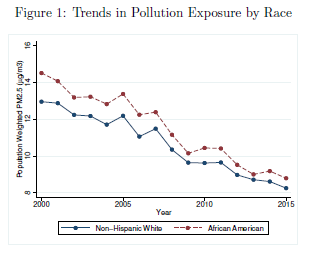
\includegraphics[scale = .5]{F1.png}
    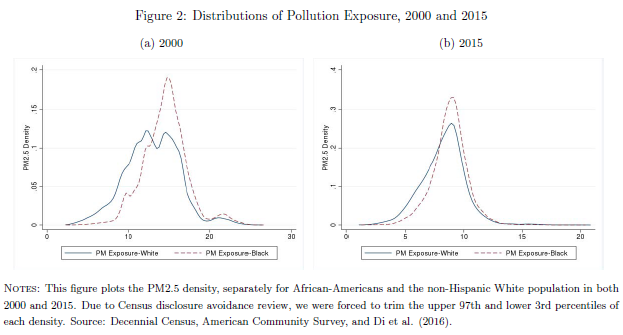
\includegraphics[scale = .5]{F2.png}
  \end{figure}
\end{frame}

\end{document}
